\documentclass[14 pt]{extarticle}

	\usepackage[frenchb]{babel}
	\usepackage[utf8]{inputenc}  
	\usepackage[T1]{fontenc}
	\usepackage{amssymb}
	\usepackage[mathscr]{euscript}
	\usepackage{stmaryrd}
	\usepackage{amsmath}
	\usepackage{tikz}
	\usepackage[all,cmtip]{xy}
	\usepackage{amsthm}
	\usepackage{varioref}
	\usepackage{geometry}
	\geometry{a4paper}
	\usepackage{lmodern}
	\usepackage{hyperref}
	\usepackage{array}
	 \usepackage{fancyhdr}
	 \usepackage{float}
\renewcommand{\theenumi}{\alph{enumi})}
	\pagestyle{fancy}
	\theoremstyle{plain}
	\fancyfoot[C]{} 
	\fancyhead[L]{Contrôle}
	\fancyhead[R]{2025-2026}\geometry{
 a4paper,
 total={190mm,257mm},
 left=9mm,
 right = 9mm,
 top=20mm,bottom = 0 mm
 }
	
	
	\title{Contrôle Chapitre 2}
	\date{}
	\begin{document}

 Nom : \\
 Prénom : 
 \subsection*{Exercice 1[sur la copie] (3 points)}
 Calculez, \emph{en détaillant les étapes} : 
 \begin{enumerate}
 \item $12 \div 2 + 2$
 \item $18 - 2 + 7$
 \item $14 \div 2 \times 7$
 \end{enumerate}
 
 \subsection*{Exercice 2[sur cette feuille] (9 points)}
 
 Tracez les symétriques de la figure suivante par rapport aux deux droites tracées, ainsi que par rapport au point E. 
 
 \begin{figure}[H]
 \center
 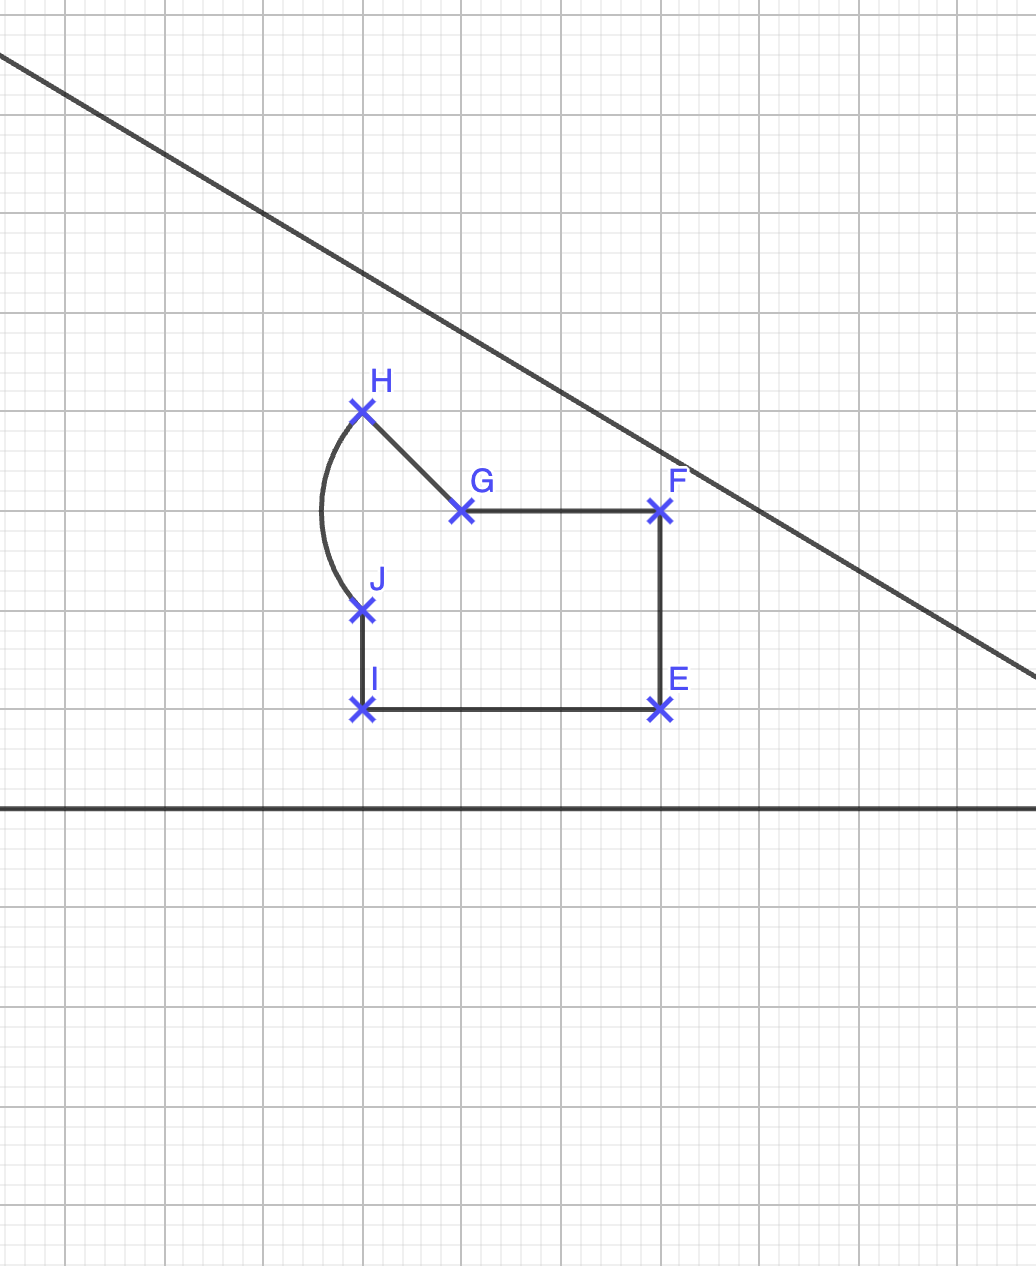
\includegraphics[width = 14.5 cm]{Fig1}
 \end{figure}

 \subsection*{Exercice 3[sur cette feuille] (3 points)}
 Dans les figures suivantes, indiquez les axes et centres de symétrie s'il y en a. 
 
 
\includegraphics[width = 5 cm]{drapeau1.png}\ \ \ \ 
 
\includegraphics[width = 5 cm]{drapeau2b.png}\ \ \ \ 
 
\includegraphics[width = 5 cm]{drapeau3.png}

 \subsection*{Exercice 4[sur votre copie] (5 points)}

On veut montrer la propriété suivante : \og Si les deux diagonales d'un quadrilatère ABCD sont perpendiculaires en leur milieu, ABCD est un losange. \fg

On considère donc un quadrilatère ABCD et on suppose que $[AC]$ et $[BD]$ se coupent en leur milieu $O$.

\begin{enumerate}
\item Justifier que $[AC]$ est la médiatrice de $[BD]$. 
\item En déduire que $B$ et $D$ sont symétriques par rapport à un axe (préciser lequel). 
\item Déduire que $BA=DA$ et $BC=DC$.
\item Utiliser une autre symétrie pour justifier que $AB=CD$, ou que $AB=AD$ (au choix).
\item En déduire que $ABCD$ est un losange. 
\end{enumerate}

\subsection*{Bonus}
Nommer les drapeaux de l'exercice 3.
\newpage


 Nom : \\
 Prénom : 
 \subsection*{Exercice 1[sur votre copie] (3 points)}
 Calculez, \emph{en détaillant les étapes} : 
 \begin{enumerate}
 \item $15 - 1 + 4$
 \item $18 \div 2 \times 9$
 \item $14 \div 2 + 7$
 \end{enumerate}
 
 \subsection*{Exercice 2[sur cette feuille] (9 points)}
 
 Tracez les symétriques de la figure suivante par rapport aux deux droites tracées, ainsi que par rapport au point E. 
 
 \begin{figure}[H]
 \center
 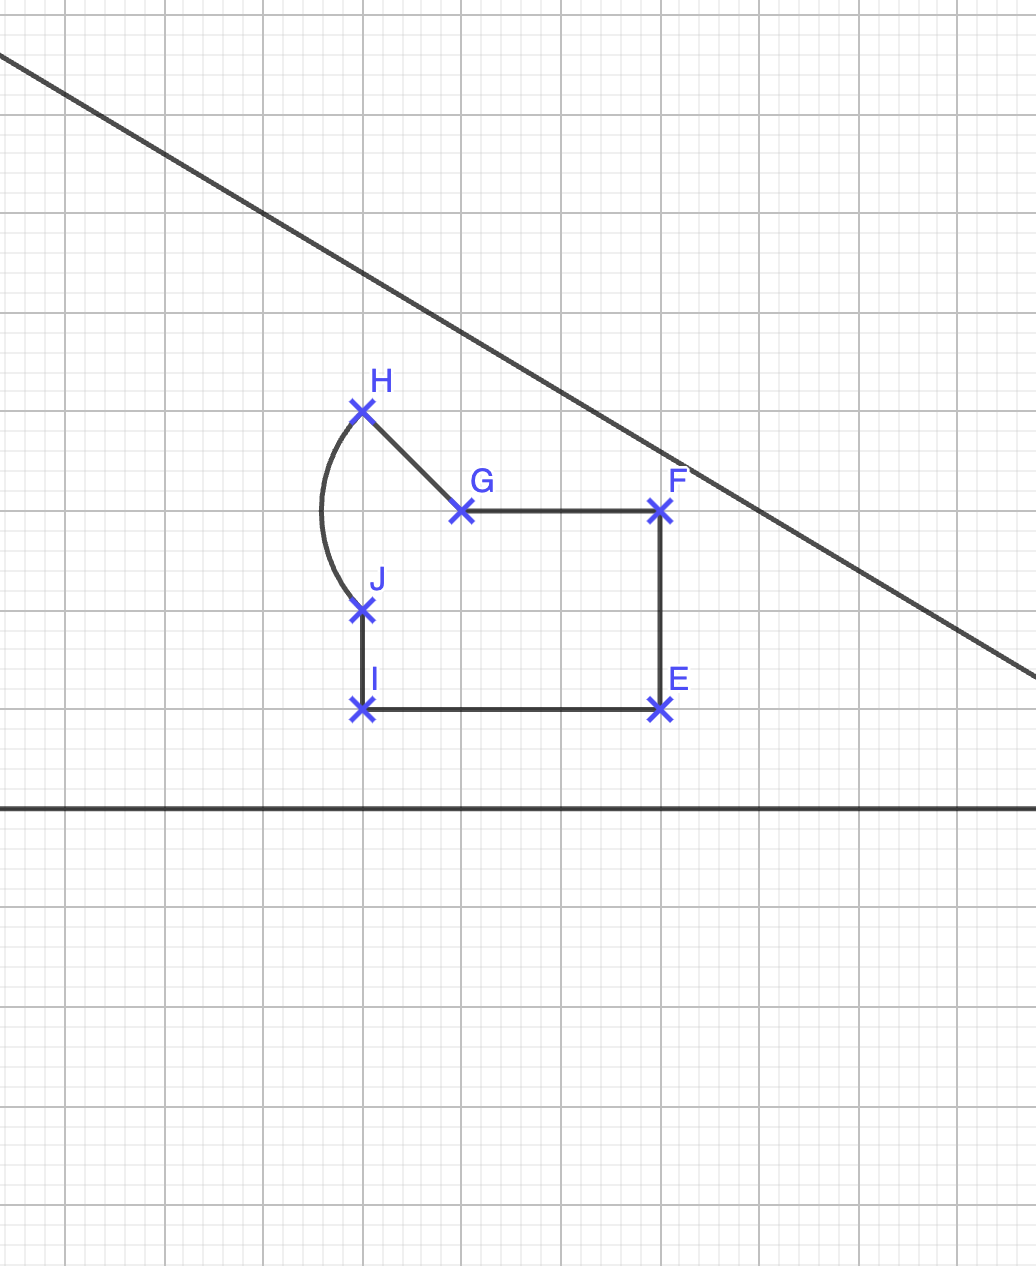
\includegraphics[width = 14.5 cm]{Fig1}
 \end{figure}

 \subsection*{Exercice 3[sur cette feuille] (3 points)}
 Dans les figures suivantes, indiquez les axes et centres de symétrie s'il y en a. 
 
 
\includegraphics[width = 5 cm]{drapeau1.png}\ \ \ \ 
 
\includegraphics[width = 6 cm]{drapeau2.png}\ \ \ \ 
 
\includegraphics[width = 4 cm]{drapeau3.png}

 \subsection*{Exercice 4[sur votre copie] (5 points)}

On veut montrer la propriété suivante : \og Si les deux diagonales d'un quadrilatère ABCD sont perpendiculaires en leur milieu, ABCD est un losange. \fg

On considère donc un quadrilatère ABCD et on suppose que $[AC]$ et $[BD]$ se coupent en leur milieu $O$.

\begin{enumerate}
\item Justifier que $[AC]$ est la médiatrice de $[BD]$. 
\item En déduire que $B$ et $D$ sont symétriques par rapport à un axe (préciser lequel). 
\item Déduire que $BA=DA$ et $BC=DC$.
\item Utiliser une autre symétrie pour justifier que $AB=CD$, ou que $AB=AD$ (au choix).
\item En déduire que $ABCD$ est un losange. 
\end{enumerate}
\subsection*{Bonus}
Nommer les drapeaux de l'exercice 3.
\newpage

 	\end{document}
